\documentclass[12pt]{article}
\usepackage[utf8]{inputenc}
\usepackage[T1]{fontenc}
\usepackage{titlesec}
\usepackage{enumitem}
\usepackage[left=2.54cm,top=3cm,right=2.54cm,bottom=3cm]{geometry}
\usepackage[sorting=none, style=numeric-comp]{biblatex}
\usepackage{hyperref}
\usepackage{graphicx}
\usepackage{upgreek}
\usepackage{setspace}
% \usepackage{longtable}
\usepackage{tabularx}
\usepackage{framed}
\usepackage{eurosym}
\usepackage{listings}
\usepackage{rotating}
\usepackage[table]{xcolor}
\usepackage[acronym,toc]{glossaries}


% \graphicspath{ {00images/} }
% \DeclareGraphicsExtensions{.png,.pdf}
% \DeclareGraphicsExtensions{.pdf,.png} % - CHANGE TO THIS

\addbibresource{mendeley.bib}
\setlength{\parindent}{1cm}

% Acronyms %%%%%%%%
\makeglossaries

\newacronym{iot}{IoT}{Internet of things}
\newacronym{gps}{GPS}{Global Positioning System}
\newacronym{gsm}{GSM}{Global System for Mobile Communication}
\newacronym{osi}{OSI}{Open Systems Interconnection}
\newacronym{mac}{MAC}{Medium Access Control}
\newacronym{llc}{LLC}{Logical Link Control}
% \newacronym{}{}{}
% \newacronym{}{}{}
% \newacronym{}{}{}
% \newacronym{}{}{}
% \newacronym{}{}{}
% \newacronym{}{}{}
% \newacronym{}{}{}
% \newacronym{}{}{}
% \newacronym{}{}{}
% \newacronym{}{}{}

\makeglossaries


%%%%%%%%%%%%%%%%%%% 

\begin{document}
% 
\tableofcontents
\pagebreak

\begin{singlespacing}
\setglossarystyle{long}
\printglossary[type=\acronymtype, title=List of acronyms and abbreviations, toctitle=List of acronyms and abbreviations, nonumberlist]
\printglossary
\end{singlespacing}

\section{Introduction}
% 
In today’s world of outsourcing production to other country than the one where the development was done in, is a common practice. Reasons varies, but mostly, it is the economical aspect. This however, raises many problems within logistics, meaning getting products from the plant on one side of the globe to a warehouses and customers on the other. Keeping track of every container leaving the plant on truck’s trailer to a port, to be loaded on a huge cargo ship with hundreds of others and subsequently being unloaded at the destination port to the right truck’s trailer and getting it to a given warehouse, poses a challenge. What is even more, as a wide range of products are being transported, each product requires a different kind of handling in means of temperature in a container, fragility of products or speed of shipment. But how to collect all of these data and provide enhanced supply chain management?
One of ways to go is the use of \acrshort{iot}\footnotemark. ``\textit{The \acrfull{iot} is a system of interrelated computing devices, mechanical and digital machines, objects, animals or people that are provided with unique identifiers and the ability to transfer data over a network without requiring human-to-human or human-to-computer interaction}'' \cite{MargaretRouse2016WhatWhatIs.com}. In the given problem in logistics, each object – container, is able to provide loads of useful data which may be collected. Collection of such data may be done with help of various sensors which may be deployed in each container. By interconnecting them, each container will have its own small network, made of several slave sensors and a master device. In this use case, the focus will be put into the use of such networks on cargo ships to provide a crew with information from each container in a central system, as well as providing a shipment client with details about his container.
% 
\footnotetext{\url{http://www.businessinsider.com/internet-of-things-logistics-supply-chain-management-2016-10?r=US&IR=T&IR=T}, accessed 05-05-2018}

To address this problem, the suggested solution is to equip each container with a hub and a set of sensors which may be added on demand, interconnecting the hub with a central receiver and providing information to a central system. In this project, the main area of research will be analysis of different wireless standards which may fit the solution as well as design of architecture of such a system.

Lets take John as an example. John is the owner of a shop chain based in Denmark, selling party decorations, costumes and gadgets. It is also a country, where their own designs are. However, as it is cheaper for them to have a production in a country with cheap work force, they are produced in China, from where all other stuff are bought as well. John would like to keep track of all containers shipped from China to Denmark, as well as being updated about conditions within container. Therefore, he decides that all of them should be equipped with \acrshort{gps}, temperature monitor, motion sensor and of course a \acrshort{gsm} module with hub. Because of that, he can track where a container is live, check whether the requested temperature for transportation is met, see when a container is being opened and have access to this information anytime and anywhere in the world. This a good solution for when a container is on land. However, when it is loaded on a cargo ship, sailing on the ocean, there is no signal from base station and therefore communication with satellite would be needed which is relatively expensive\footnotemark.
% 
\footnotetext{\url{https://www.quora.com/Why-is-satellite-Internet-service-so-relatively-expensive-and-not-available-worldwide}, accessed 05-05-2018}

One of many solutions to this problem, would be having a cargo ship equipped with several hubs to which containers on board would be periodically pushing information and these will be collected in the central system. This information then, would be every few minutes sent via satellite to central server and accessible for a client. Because of that, the cost for internet connection on board would be lower as there would be only one from the central system instead of many from each container, and crew would have precise information about each container, knowing if there was some problem.
\section{Architecture}

The main actors in the system are clear: the heart of the problem is the temperature-sensitive cargo that needs to be transported. This cargo is loaded in the refrigerated containers, also known as reefers. Each type of cargo requires different temperature and air composition, so these settings differ among the reefers. There is at least one temperature sensor and one gas monitoring sensor in every reefer. Reefers, together with regular containers and other cargo are loaded onto a vessel and transported across the sea.

When the temperature and the air quality are monitored, the goal is to transfer the data to:

\begin{itemize}
    \item \textit{Collection point/database}, so that the transport company can prove to its customers that the cargo maintained the desired temperature throughout the whole duration of the journey. Some systems allow the customer to monitor the data from the container in real time.
    \item \textit{Ship bridge}, to ensure that the temperature in the container is not too high (i.e. due to a power loss) and that the systems are operating normally (i.e. there is no fire in the container). 
\end{itemize}

The simplest architecture for this transfer of data from every container would probably consist of sensors submitting data directly to the collection point. It is obvious that this probably has many drawbacks. Even if there are only two sensors in each containers, there are still hundreds of containers on a ship. If there was only one collection point for all of Maersk’s fleet, this point would need to handle connections from tens of thousands devices, since there are hundreds of ships in operation worldwide.

//THIS IS SHOWN IN FIGURE

A solution to this problem is to introduce a \textit{hub}. Hub is a cluster node, that collects, processes and re-transmits data to the sink, but it does not sense any data by itself. The sensors in the container would connect to a hub and the hub would then connect to sink. This reduces the number of connections that need to be handled by the sink and also limits the necessary transmission power of the sensor. The problem then lies in the relative position of the hub. If the hub is positioned too close to the sensors, we can lower the necessary transmission power of the sensors, but more hubs per vessel would be needed to cover all of the containers. If the hub is too far from the sensors, less hubs per vessel would be needed, but the range of the sensors would need to increase. The lesser the hubs are there, the fewer communication links to the sink are needed. In a shipping scenario, where vessels are often out of reach of the traditional \acrshort{gsm} band and satellite communication must be used to transmit data to shore. Satellite link is a scarce resource and limiting the amount of satellite connections required is beneficial.

//SHOWN IN A FIGURE TOO, I GUESS

An alternative solution to compromise between the sensor transmit power and number of hubs required, is to introduce a second-level hub. Second-level hubs are the middle man between first-level hubs and the sink. Sensors connect and transfer their data to the first-level hub. This hub processes the data and forwards it to the second-level hub. Second-level hub collects the data and forwards them to the sink in batches. A plausible placements of the hubs could be inside a container for the first-level hub and on the bridge for the second-level hub. In this setup, the sensors only need to transmit their data over a short distance, therefore the power consumption can be reduced. The second-level hub collects data from the whole vessel before forwarding them to the sink. If there only is one second-level hub per vessel, the number of satellite links required is reduced.
%
% 
% \footnotetext{This does not neccessarily refer to the physical distance to the sensors, rather than relative position in the architecture with respect to}

\subsection{Data link layer}
Data link layer is the second layer of the \acrshort{osi} reference model. It consists of \acrfull{mac} and \acrfull{llc} layer. The \acrshort{mac} layer is responsible for regulating the access to the shared communication medium among nodes, while the \acrshort{llc} layer is used to define and control properties of the \acrshort{mac} layer, to shield the upper layers of the model from the physical network and provide inter-operability  across different types of networks. Since the use of \acrshort{llc} layer in practice is limited~\cite{Sohraby2007WirelessApplications}, we will further focus on the \acrshort{mac} layer.

The medium access control layer is responsible for managing the access to the shared communication medium. In wireless networks, it is usually the case that only one device can use the wireless medium at a time, otherwise the interference of wireless signals will render the transmission invalid. The \acrshort{mac} layer resolves this problem, by maintaining a scheme on how and when each node can transmit. The design of the \acrshort{mac} layer is the ``\textit{major determining factor in Wireless Sensor Network performance}''\cite{Sohraby2007WirelessApplications}. 

However, there are several complexities associated with designing this layer. Besides the overall complexity spanning through the whole system, such as limited performance of the devices due to size and power constraints, \acrshort{mac} layer must also account for eventual movement of the devices. Furthermore, when the \acrshort{mac} layer needs to coordinate access to a medium, often the same medium must also be used for this coordination effort. This coordination effort results in better decisions of nodes when to transmit and when not to. The better the decisions, the fewer collisions appear and the less wasted time and transmission power. However, this coordination effort imposes overhead on the communication channel -- on top of the actual data from the sensors, some sort of coordination needs to be added. As~\cite{Sohraby2007WirelessApplications} notes, a trade-off between the quality of the decision and the amount of overhead incurred needs to be made.

There are several metrics that can be used to asses the performance of a \acrshort{mac} layer. 

\begin{table}[ht]
    \centering
    \begin{tabularx}{\textwidth}{|l|X|p{5em}|}
    \hline
    \textbf{Metrics}&\textbf{Description}&\textbf{Relevance}\\
    \hline
    Delay&Sohraby et. al. defines delay as the amount of time packet spends in the MAC layer before it is transmitted successfully~\cite{Sohraby2007WirelessApplications}.&•\\
    \hline
    Throughput&Throughput is the rate of successful message delivery through the communication channel.&•\\
    \hline
    Scalability&Scalability is the ability of the protocol to maintain its usual performance with increasing amount of devices&•••\\
    \hline
    Stability&Stability is a metrics that measures how well can the system resist changes of the traffic load over a period of time.&•••\\
    \hline
    Fairness&Fairness of a MAC protocol describes how well does the protocol distribute resources among the devices without significantly limiting the throughput.&••\\
    \hline
    \end{tabularx}
    \caption{Comparison of different MAC layer metrics. The \textit{Relevance} column is an approximation of how relevant this metric is in the reefer shipping scenario.}
    \label{tab:mac-metrics}
\end{table}

Generally, the MAC protocols can be divided into two groups: contention-free and contention-based protocols. Contention-free protocols only allow one device to access the medium at the time. This group can be further divided into \textit{fixed assignment} and \textit{dynamic assignment}, depending on how the protocol assigns communication slots to devices. Contention-based protocols allow multiple devices to access the medium at the same time, but provide a recovery mechanism, shall a collision occur. Figure~\ref{fig:mac-categories} displays this grouping.

\begin{figure}[ht]
    \centering
    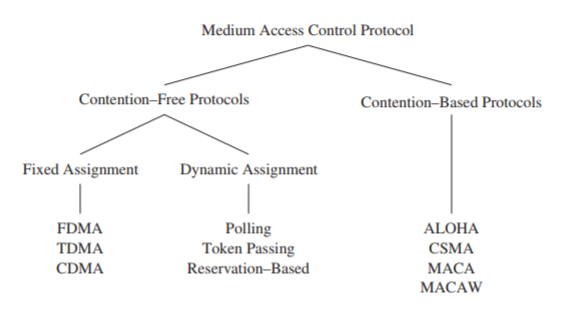
\includegraphics[width=0.8\textwidth]{00images/mac-categories}
    \caption{Categorisation of MAC protocols, according to channel access. Few examples are given for each category. Taken from~\cite{2011MediumControl}.}
    \label{fig:mac-categories}
\end{figure}
\pagebreak


\printbibliography[heading=bibintoc]
\pagebreak


\end{document}
